\subsubsection{Functional Requirements}
\begin{itemize}
  \item The system shall charge the user using her payment information after each utilization.
  \item The system shall start to calculate the charge as soon as the engine ignites.
  \item The system shall stop to calculate the final charge as soon as the car is parked in a safe area and the user exits the car.%same moment that the car is locked
  \item The system shall start to calculate the charge as soon as the engine ignites.
  \item The system shall calculate the current charges. The amount of money per minute is gived.
  \item The system shall notified the current charges to the user through a screen on the car.
\end{itemize}

\subsubsection{Scenario 1}
Mark has just used PowerEnJoy for going from his house to his office. During his travel he frequently check the car's monitor in order to know the amount of the current charges. When he arrives in a park near his office, which is in a safe area, he turns off the engine and exits the car. At this point the system automatically lock the car and stops charging Mark. After a while Mark receives a notification by the system about the last ride, with travel information and the final charge. The bank inform Mark that the charge was applied on his bank account. 


\subsubsection{Scenario 2}
During a sunny day Susan decides to use PowerEnJoy to go to the countryside. She takes a car and drives for an hour. When she arrives she notices that the system doesn't stop to charge her. After a quick check she discovers that it isn't a safe area. Unfortunatly for stopping the charge she has to drive back for a while and park the car in a safe area. She finds a bus and uses it for reach the countryside again. The PowerEnJoy service should be used mostly for travels around the city, the cars should be available alongside the city ready for being shared between the users. 

%\subsubsection{Mockups}
%\begin{figure}[!ht]
%  \centering
 % \vspace{0.2cm}
 % 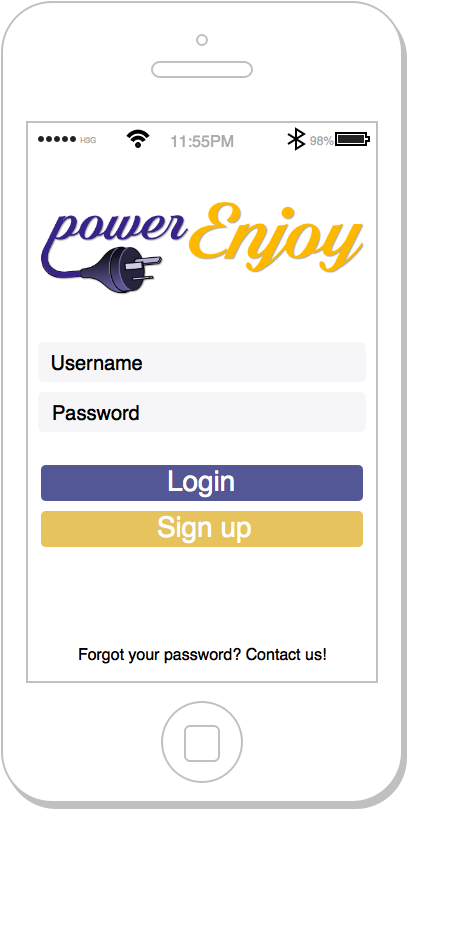
\includegraphics[width=0.25\textwidth]{/RASD/System_Functions/login_mockup}\\
 % \vspace{0.4cm}
  %\caption{Mockup for the login mobile page} 
 % \label{fig:login_mockup} 
%\end{figure}
% maybe home page mockup here 


\subsubsection{Use-case table}
\begin{center}
  \begin{tabular}{ l | p{10cm} }
    \hline
    Actors & User\\ \hline
    Goal & G\ref{itm:goal-payment}\\ \hline
    Entry conditions & 
    \begin{itemize}
    %\item The User has unlocked a car.
   % \item The User is on-board.
    \item The user has turns off the engine and exits the car.
    \item The system stops charging the user and locks the car.
    \end{itemize} \\ \hline
    Flow of events &
\begin{itemize}
%\item The engine ignites and the system start charging the User.
%\item The User starts to drive. 
%\item The user is notified of the current charges through a screen on the car.
\item The system check the car location.
\item The system notify the user about her final charge.
\item The User does the payment.
\item The system notify the success of the payment
\end{itemize} \\ \hline
    Exit conditions & The User has finished his ride and has payed PowerEnJoy for the service. \\ \hline
  Exceptions & 
\begin{itemize}
\item The payment failed.
\item The User turns off the engine and exits the car in a not safe area
\item The system is not able to complete the operation due to some internal issues or connection broken (the system signals a ConnectionFailure).%volendo si possono modificare i nomi delle eccezzioni.
\end{itemize} \\ \hline
  \end{tabular}
\end{center}


\subsubsection{Sequence diagram}
\begin{figure}[!ht]
  \centering
  \vspace{0.1cm}
  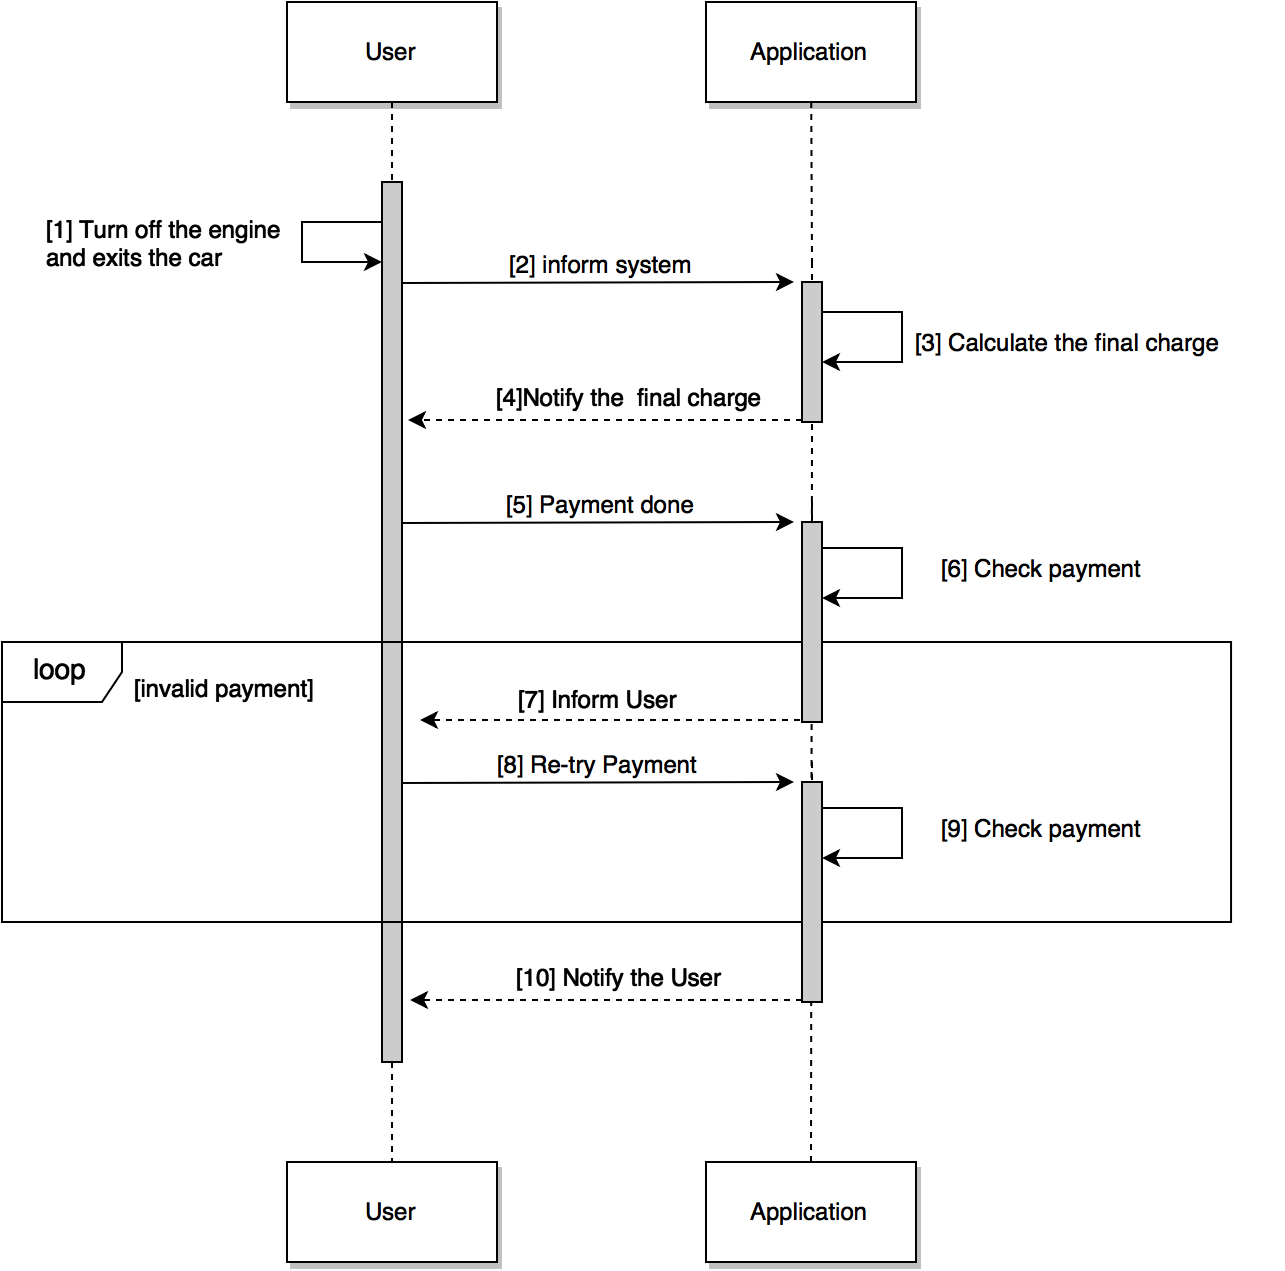
\includegraphics[width=0.6\textwidth]{/RASD/System_Functions/charge_sequence}\\
  \vspace{0.1cm}
  %\caption{Sequence diagram for the login procedure} 
  \label{fig:charge_sequence} 
\end{figure}

